
\begin{frame}{Движение 1 ($\nu_{1,2}(0) = 0, \nu_3 = 1$).}
    \begin{figure}[H]
        \centering
        \begin{columns}
            \column{0.33\textwidth}
                \centering
                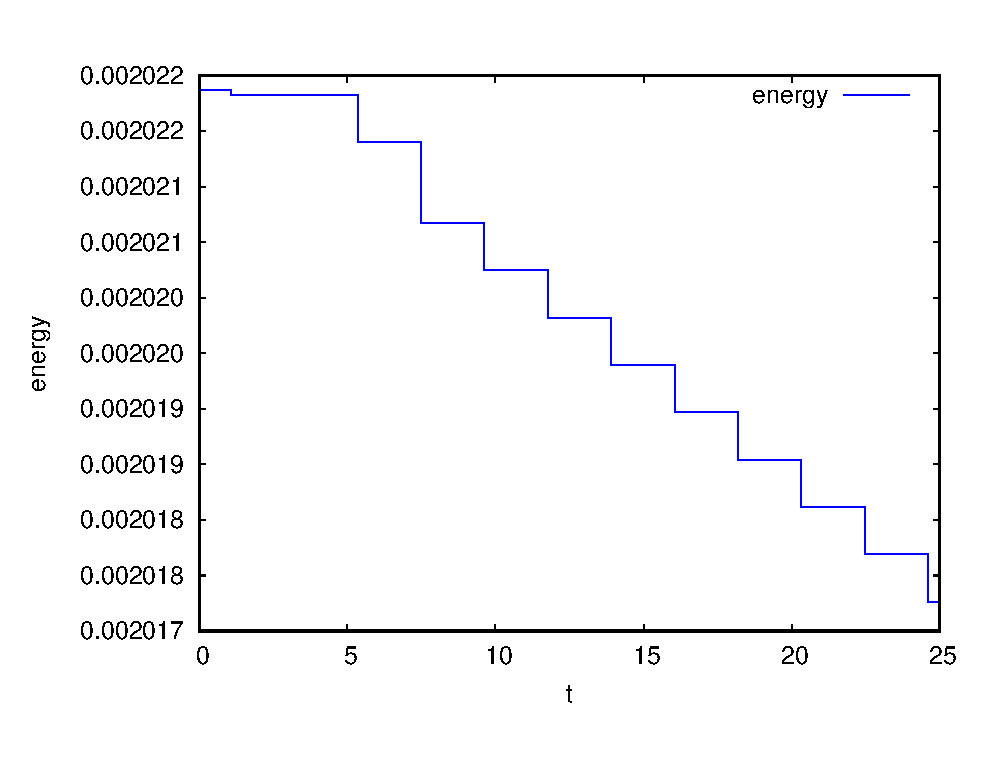
\includegraphics[width=\linewidth]{content/pic/self_rot_25/kin_en.eps}
                \vspace{-15pt}
                \caption{Кинетическая энергия}
            \column{0.33\textwidth}
                \centering
                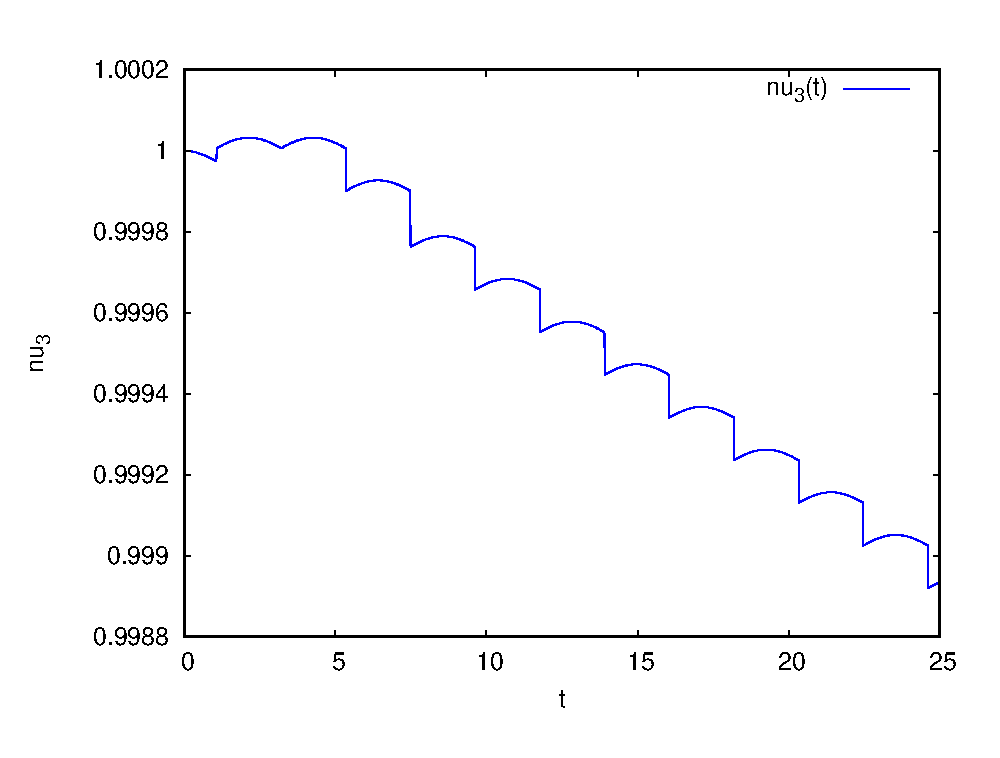
\includegraphics[width=\linewidth]{content/pic/self_rot_25/nu3.eps}
                \vspace{-15pt}
                \caption{Угловая скорость экипажа}
            \column{0.33\textwidth}
                \centering
                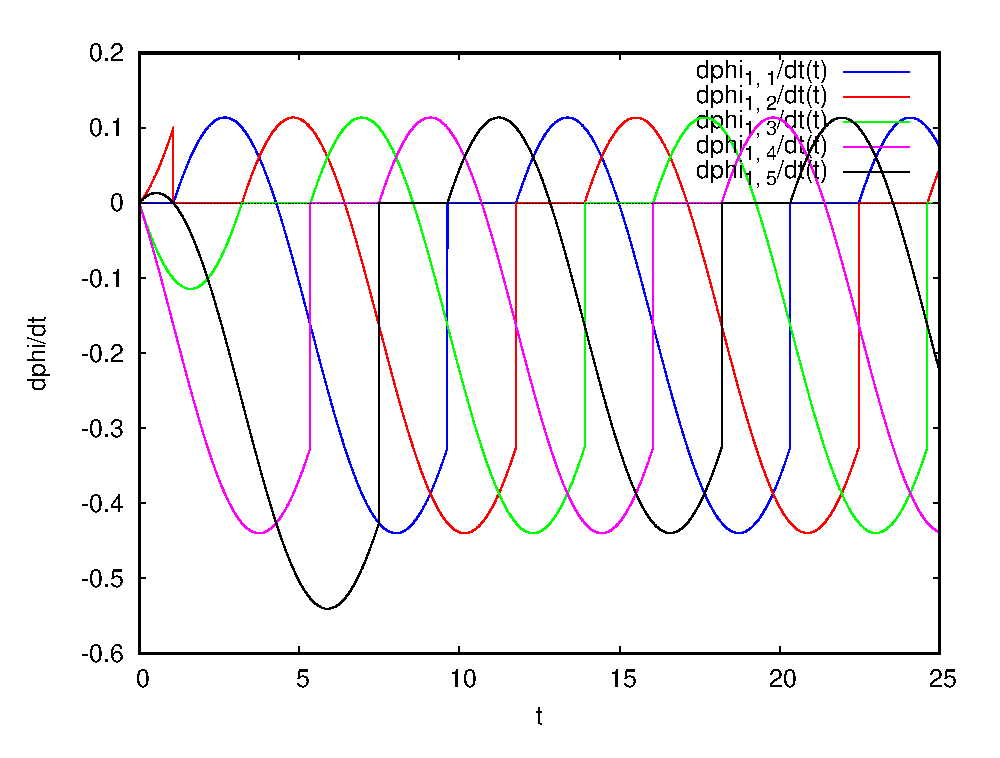
\includegraphics[width=\linewidth]{content/pic/self_rot_25/rol_vel.eps}
                \vspace{-15pt}
                \caption{Угловые скорости роликов}
        \end{columns}
    \end{figure}
    % \vspace{-25pt}
    % \begin{figure}[H]
    %     \centering
    %     \begin{columns}
    %         \column{0.33\textwidth}
    %             \centering
    %             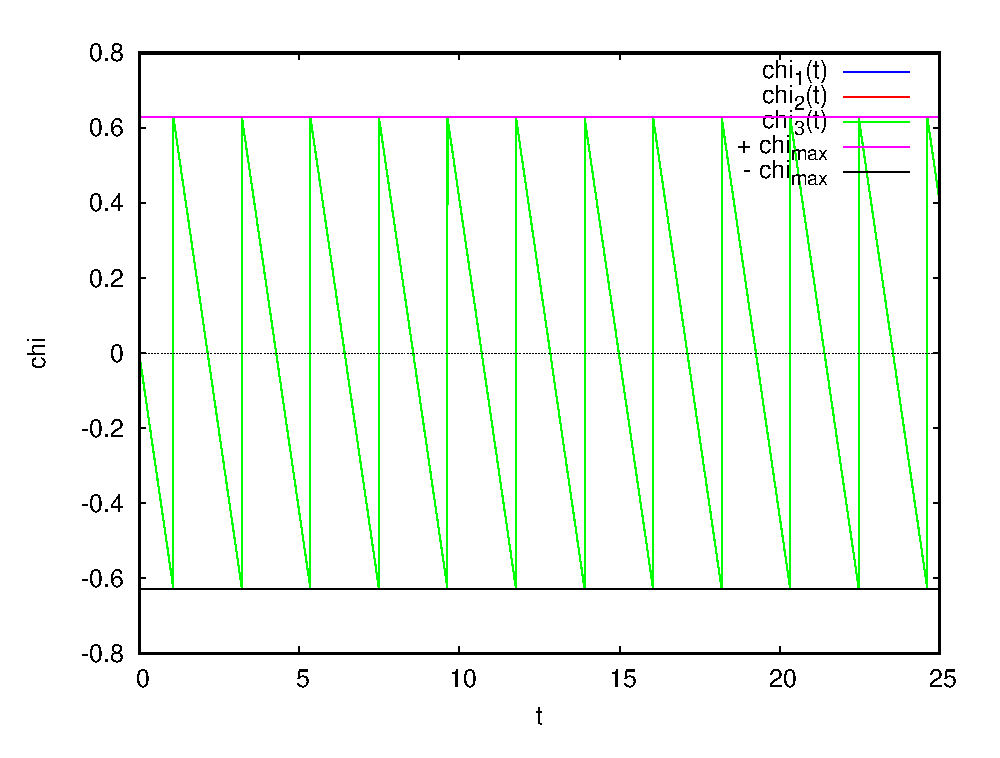
\includegraphics[width=\linewidth]{content/pic/self_rot_25/chi.eps}
    %             \vspace{-15pt}
    %             \caption{Углы поворота колес}
    %         \column{0.33\textwidth}
    %             \centering
    %             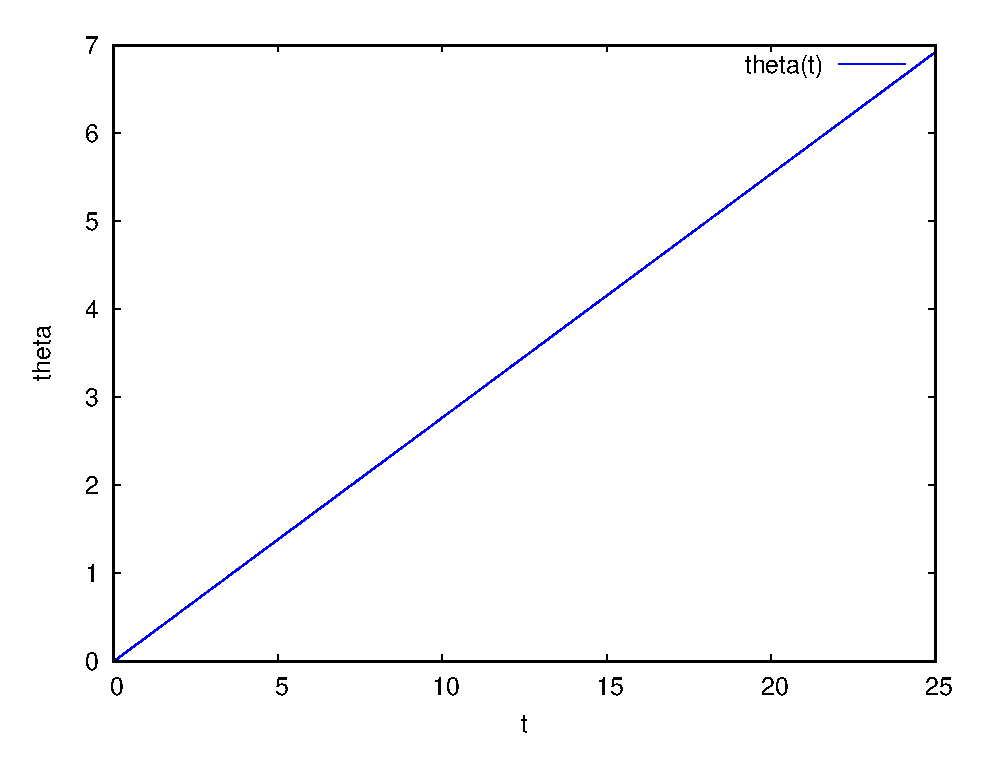
\includegraphics[width=\linewidth]{content/pic/self_rot_25/theta.eps}
    %             \vspace{-15pt}
    %             \caption{Угол поворота экипажа}
    %         \column{0.33\textwidth}
    %             \centering
    %             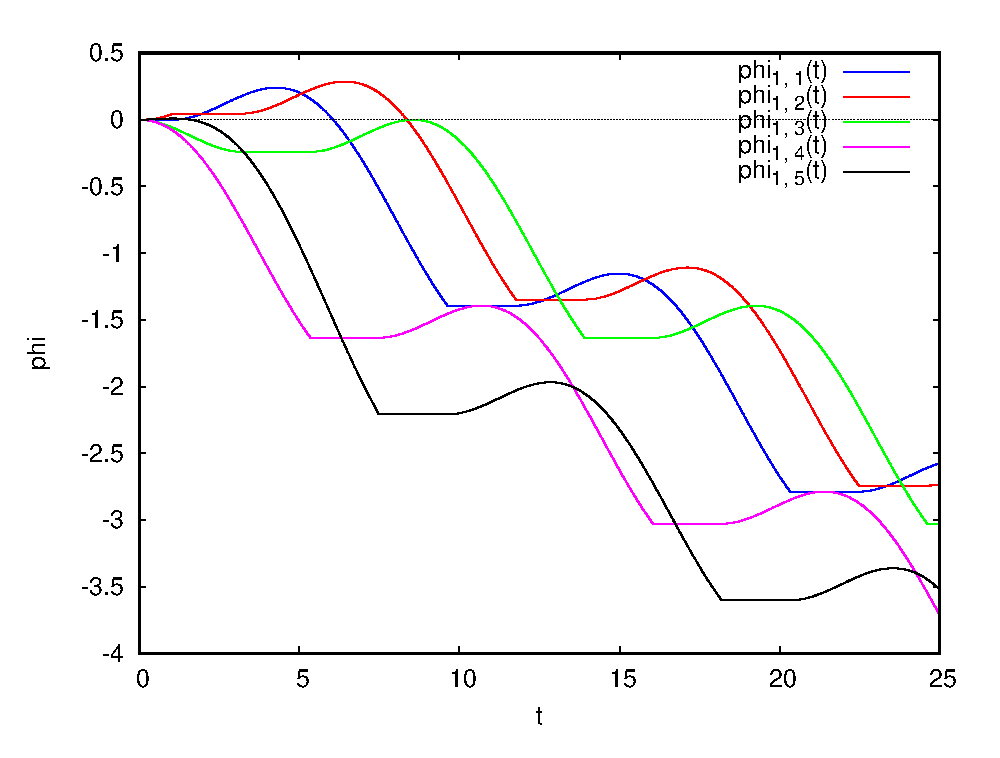
\includegraphics[width=\linewidth]{content/pic/self_rot_25/rol_ang.eps}
    %             \vspace{-15pt}
    %             \caption{Углы поворота роликов}
    %     \end{columns}
    % \end{figure}
\end{frame}

\begin{frame}{Движение 2 ($\nu_1(0) = 1, \nu_{2,3} = 0$).}
    % \begin{figure}[H]
    %     \centering
    %     \begin{columns}
    %         % \column{0.25\textwidth}
    %         \column{0.25\textwidth}
    %             \centering
    %             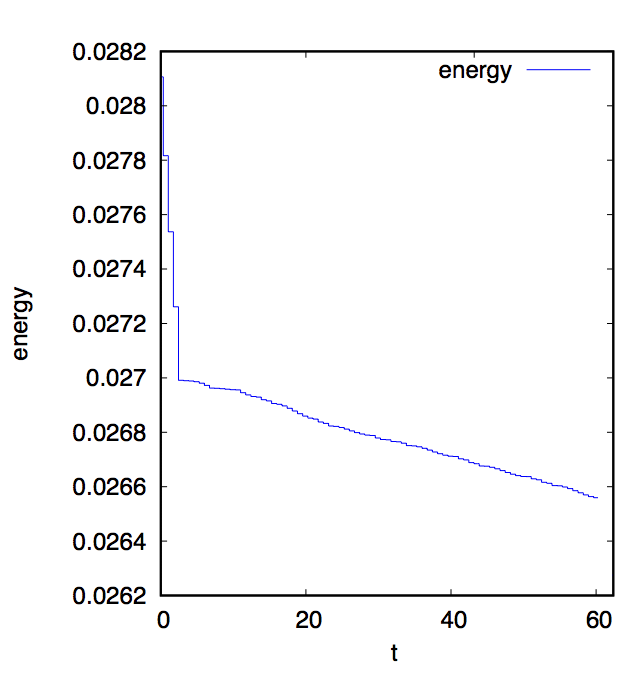
\includegraphics[width=1.1\linewidth]{content/pic/straight_60/kin_en.png}
    %             \vspace{-15pt}
    %             \caption{Кинетическая энергия}
    %         % \column{0.37\textwidth}
    %         \column{0.37\textwidth}
    %             \centering
    %             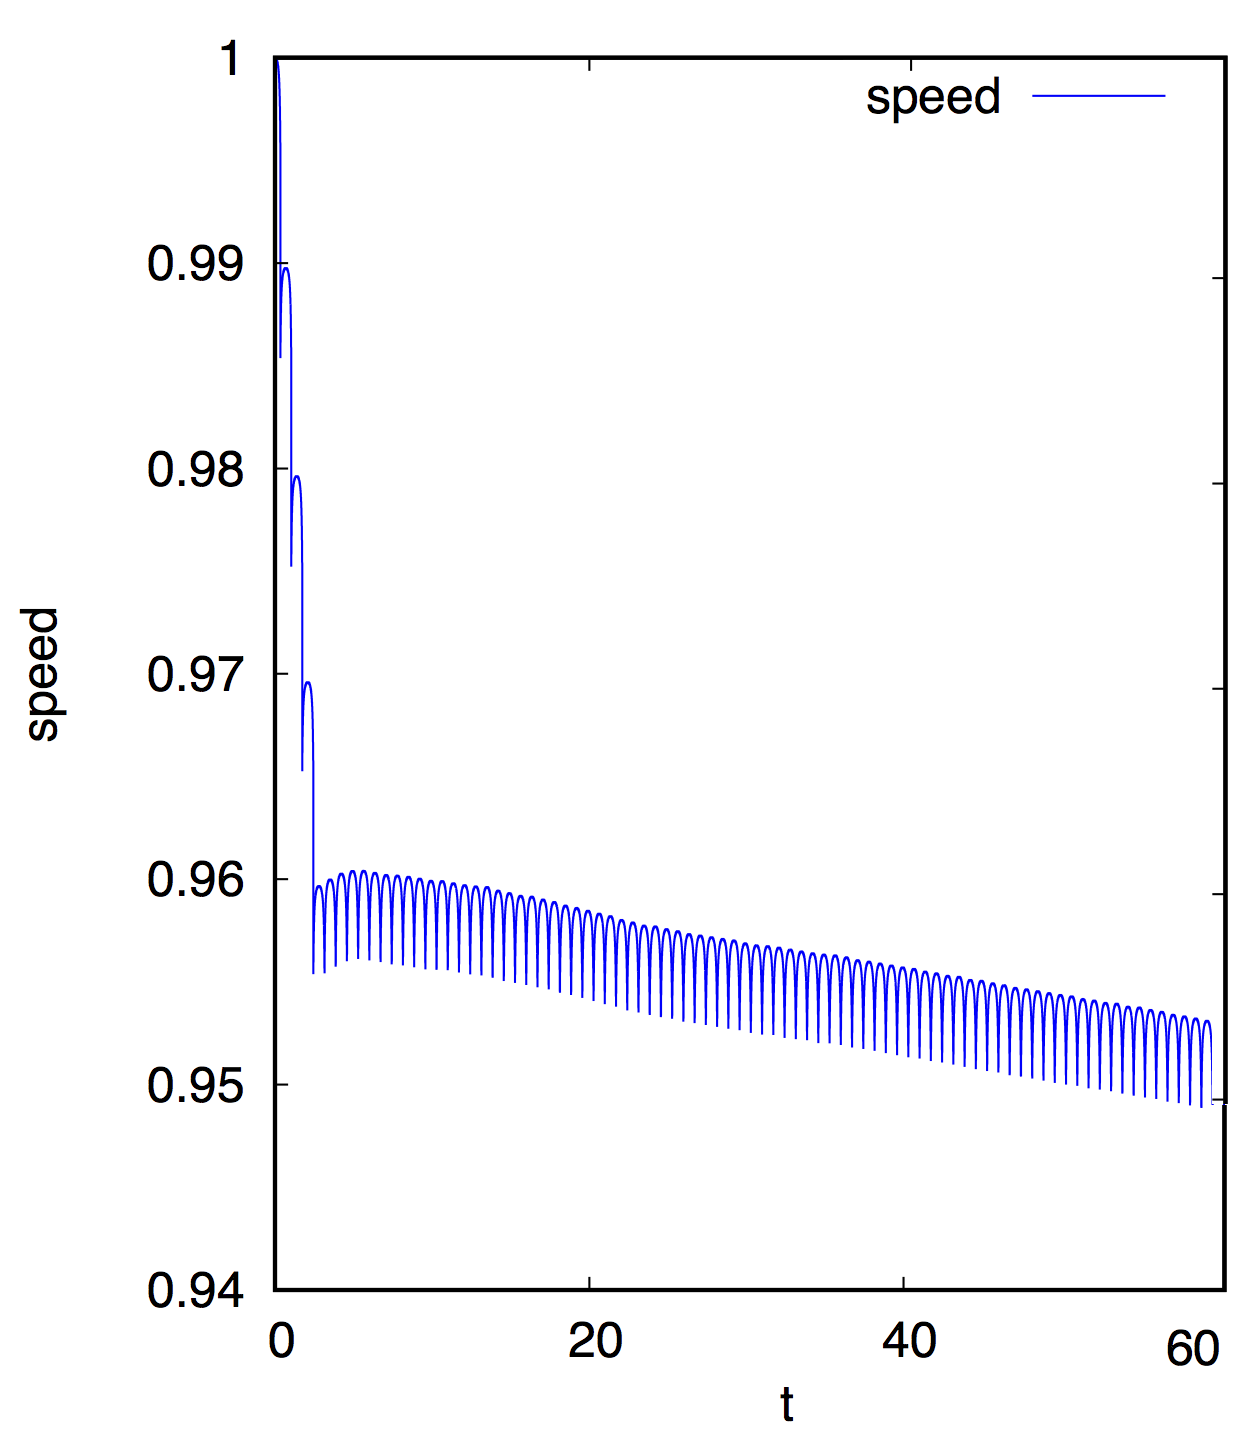
\includegraphics[width=0.8\linewidth]{content/pic/straight_60/v.png}
    %             \vspace{-15pt}
    %             \caption{Скорость центра масс}
    %         % \column{0.37\textwidth}
    %         %     \centering
    %         %     \vspace{2.5pt}
    %         %     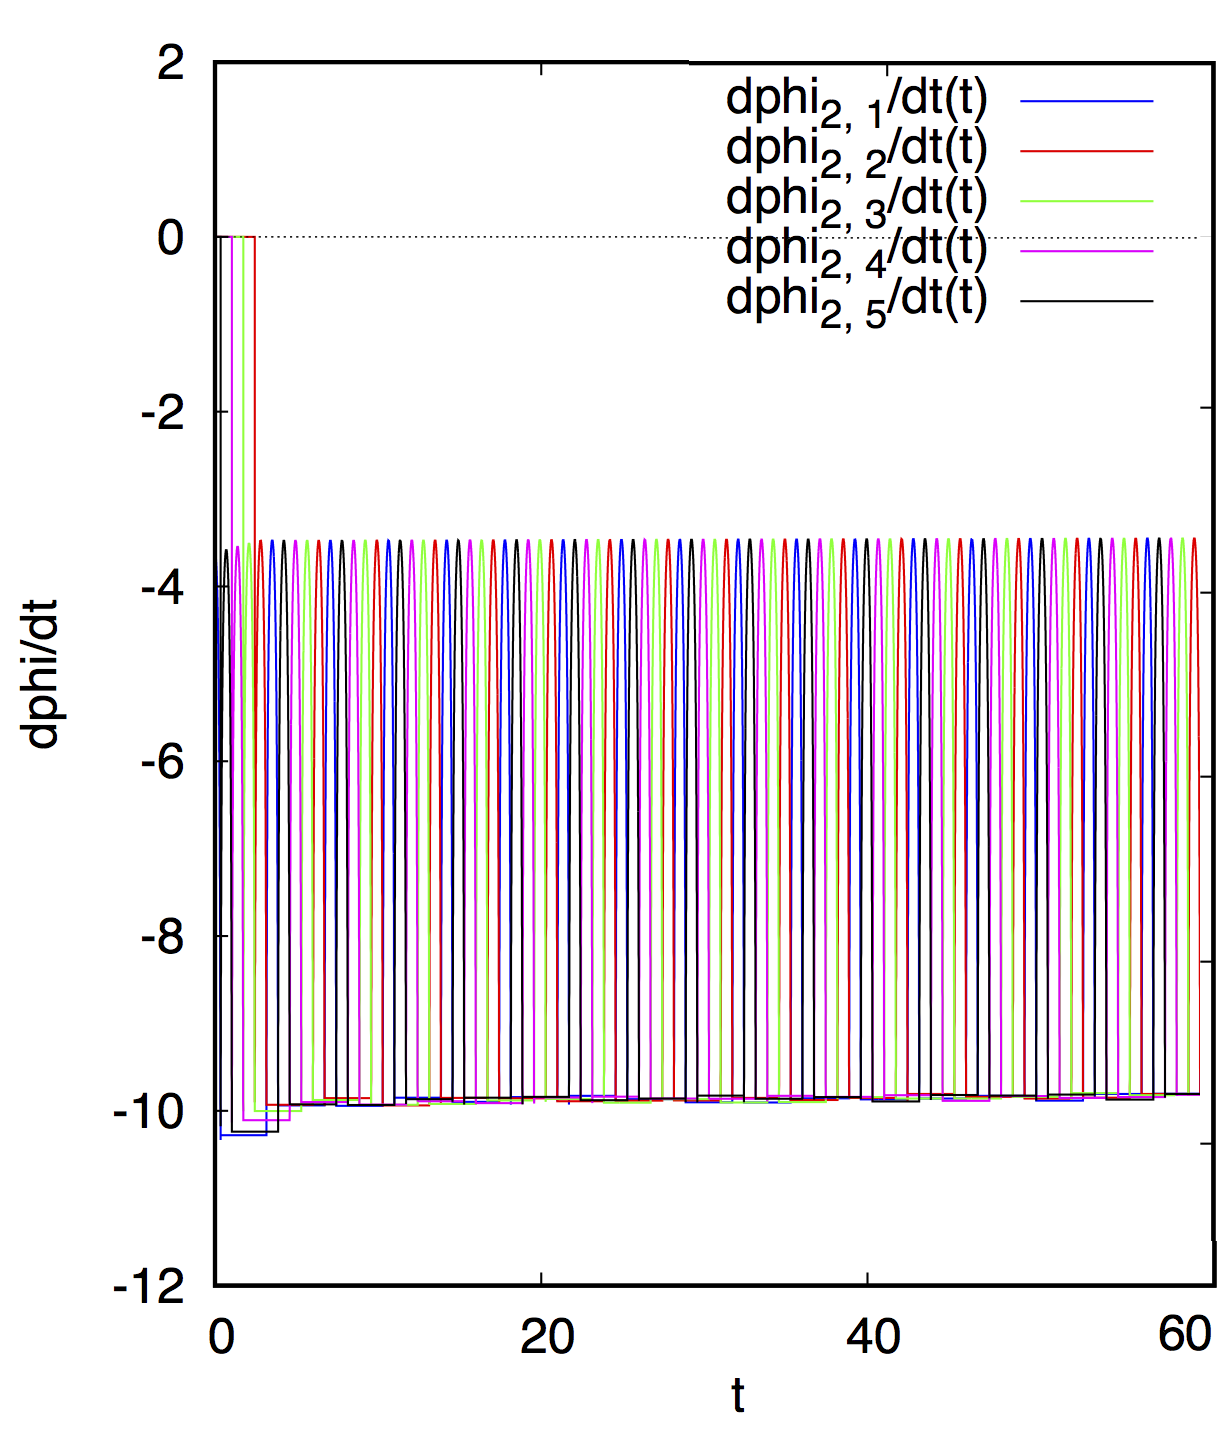
\includegraphics[width=0.8\linewidth]{content/pic/straight_60/nus2.png}
    %         %     \vspace{-15pt}
    %         %     \caption{$\dot{\mathbf{\phi}}$ на заднем колесе}
    %     \end{columns}
    % \end{figure}
    % \vspace{-25pt}
    % \begin{figure}[H]
    %     \centering
    %     \begin{columns}
    %         \column{0.33\textwidth}
    %             \centering
    %             \vspace{2.5pt}
    %             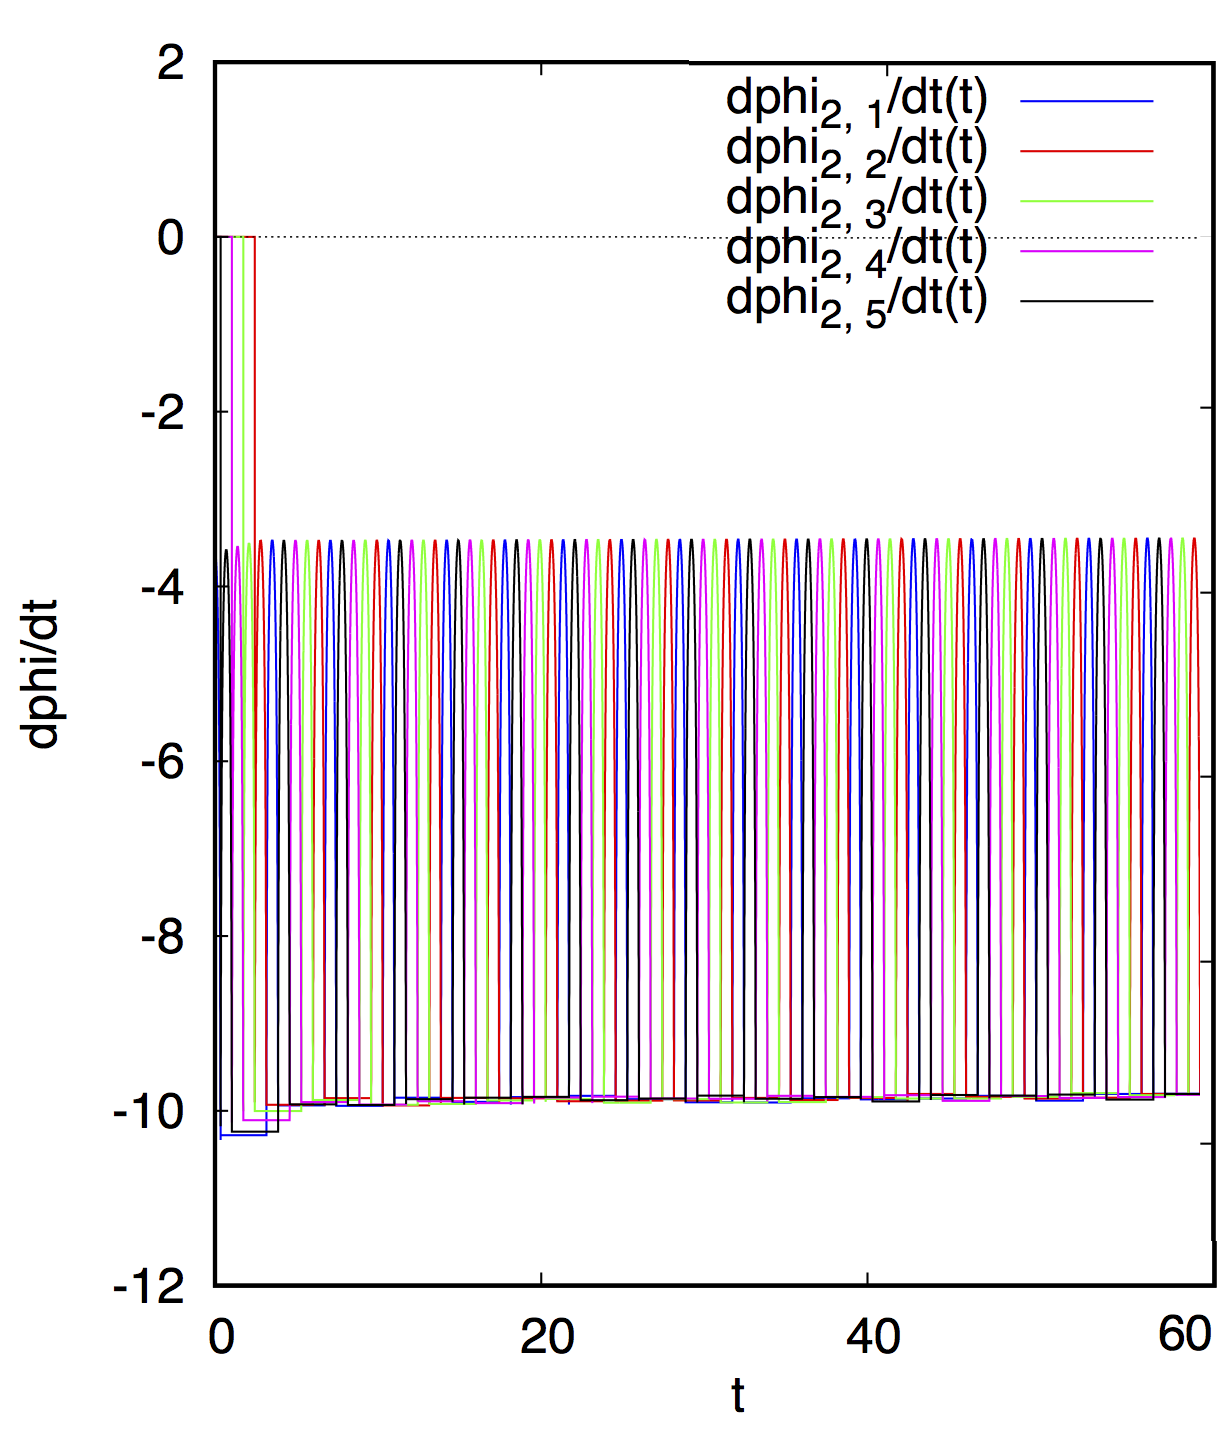
\includegraphics[width=0.8\linewidth]{content/pic/straight_60/nus2.png}
    %             \vspace{-15pt}
    %             \caption{$\dot{\mathbf{\phi}}$ на заднем колесе}
    %         % \column{0.33\textwidth}
    %         %     \centering
    %         %     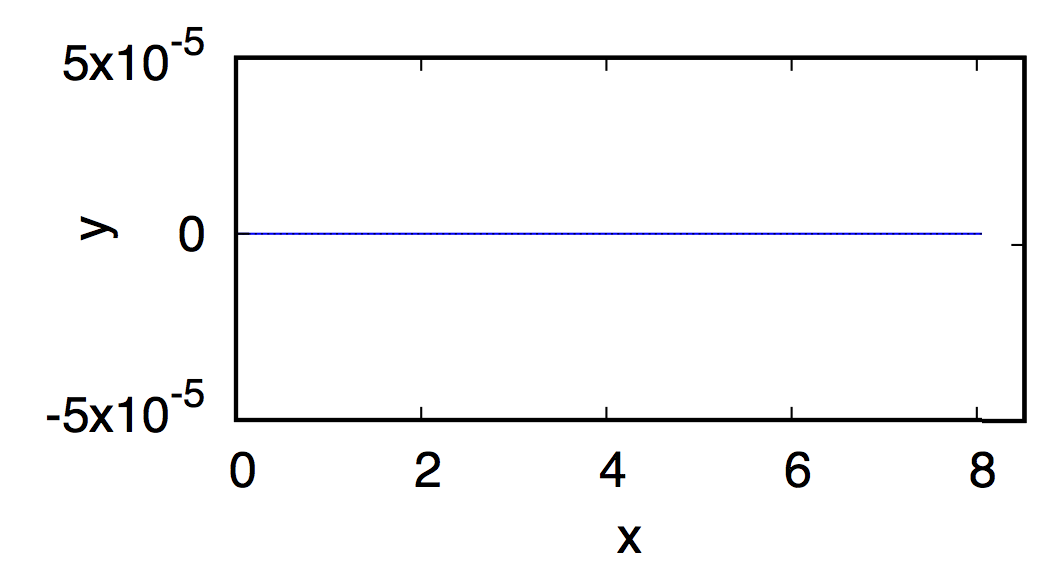
\includegraphics[width=\linewidth]{content/pic/straight_60/traj.png}
    %         %     \vspace{-15pt}
    %         %     \caption{Траектория}
    %         % \column{0.33\textwidth}
    %         %     \centering
    %         %     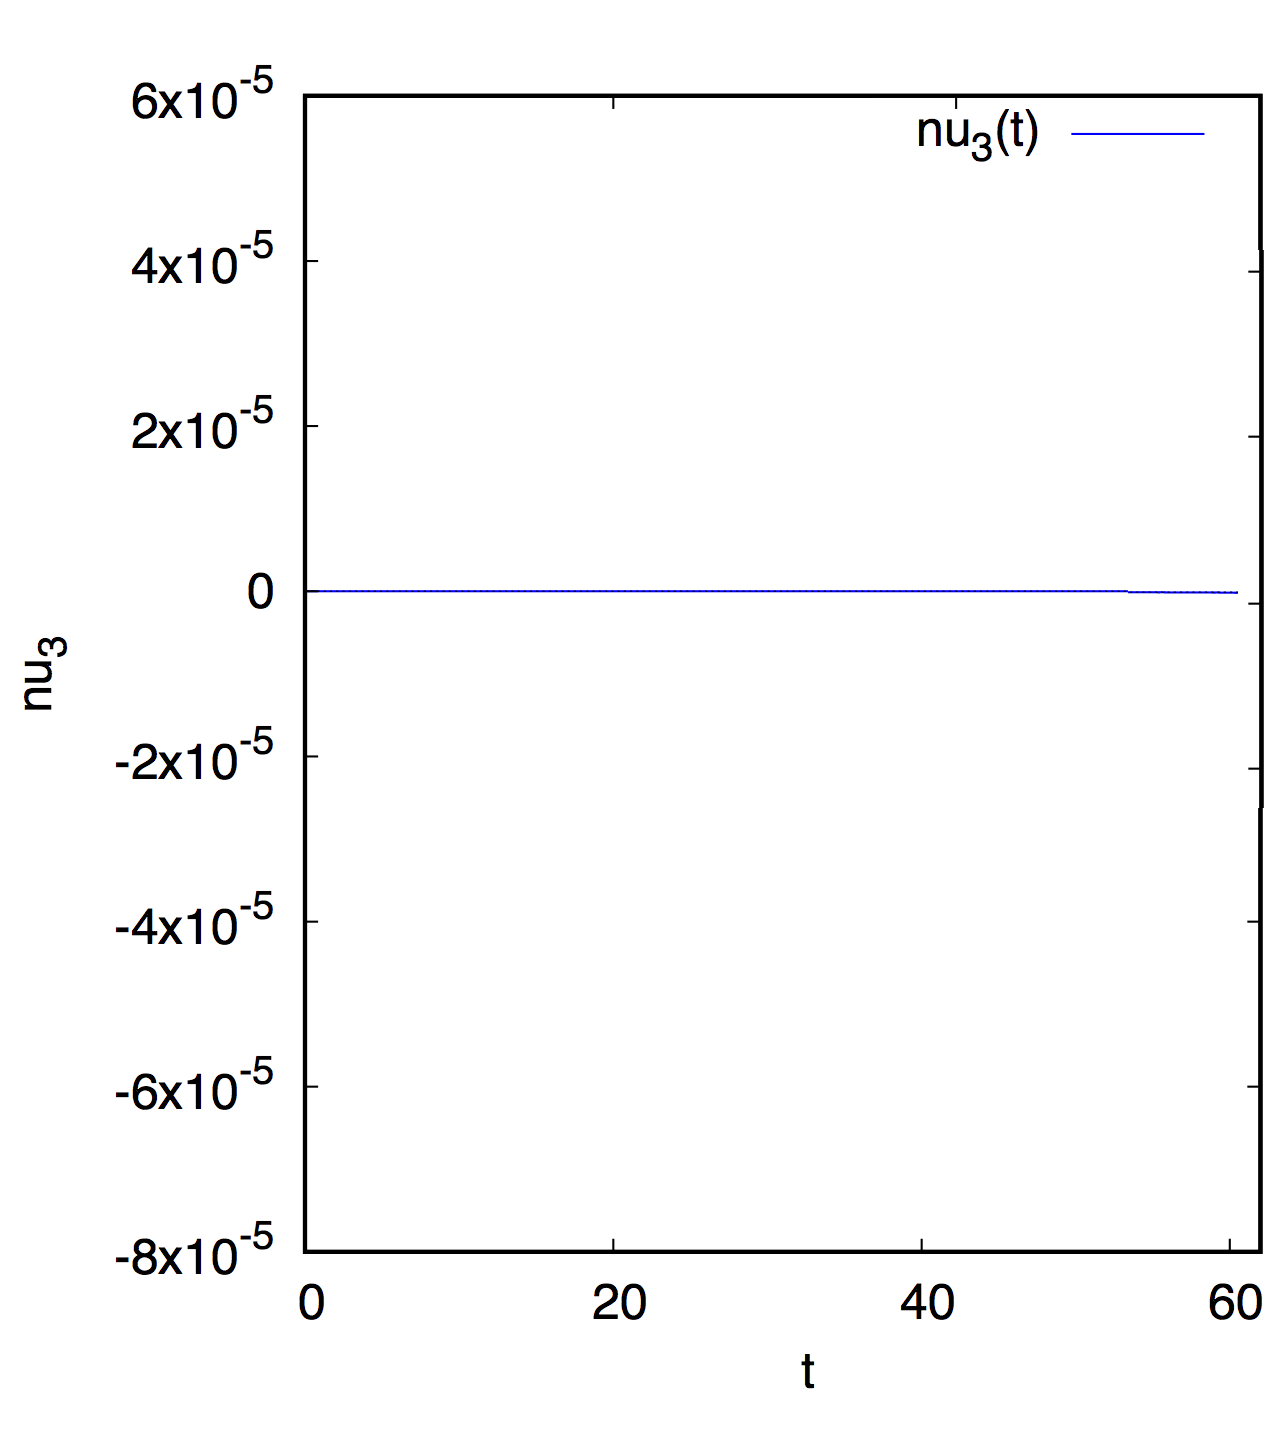
\includegraphics[width=0.8\linewidth]{content/pic/straight_60/nu3.png}
    %         %     \vspace{-15pt}
    %         %     \caption{Угловая скорость экипажа}
    %         % \column{0.33\textwidth}
    %         \column{0.33\textwidth}
    %             \centering
    %             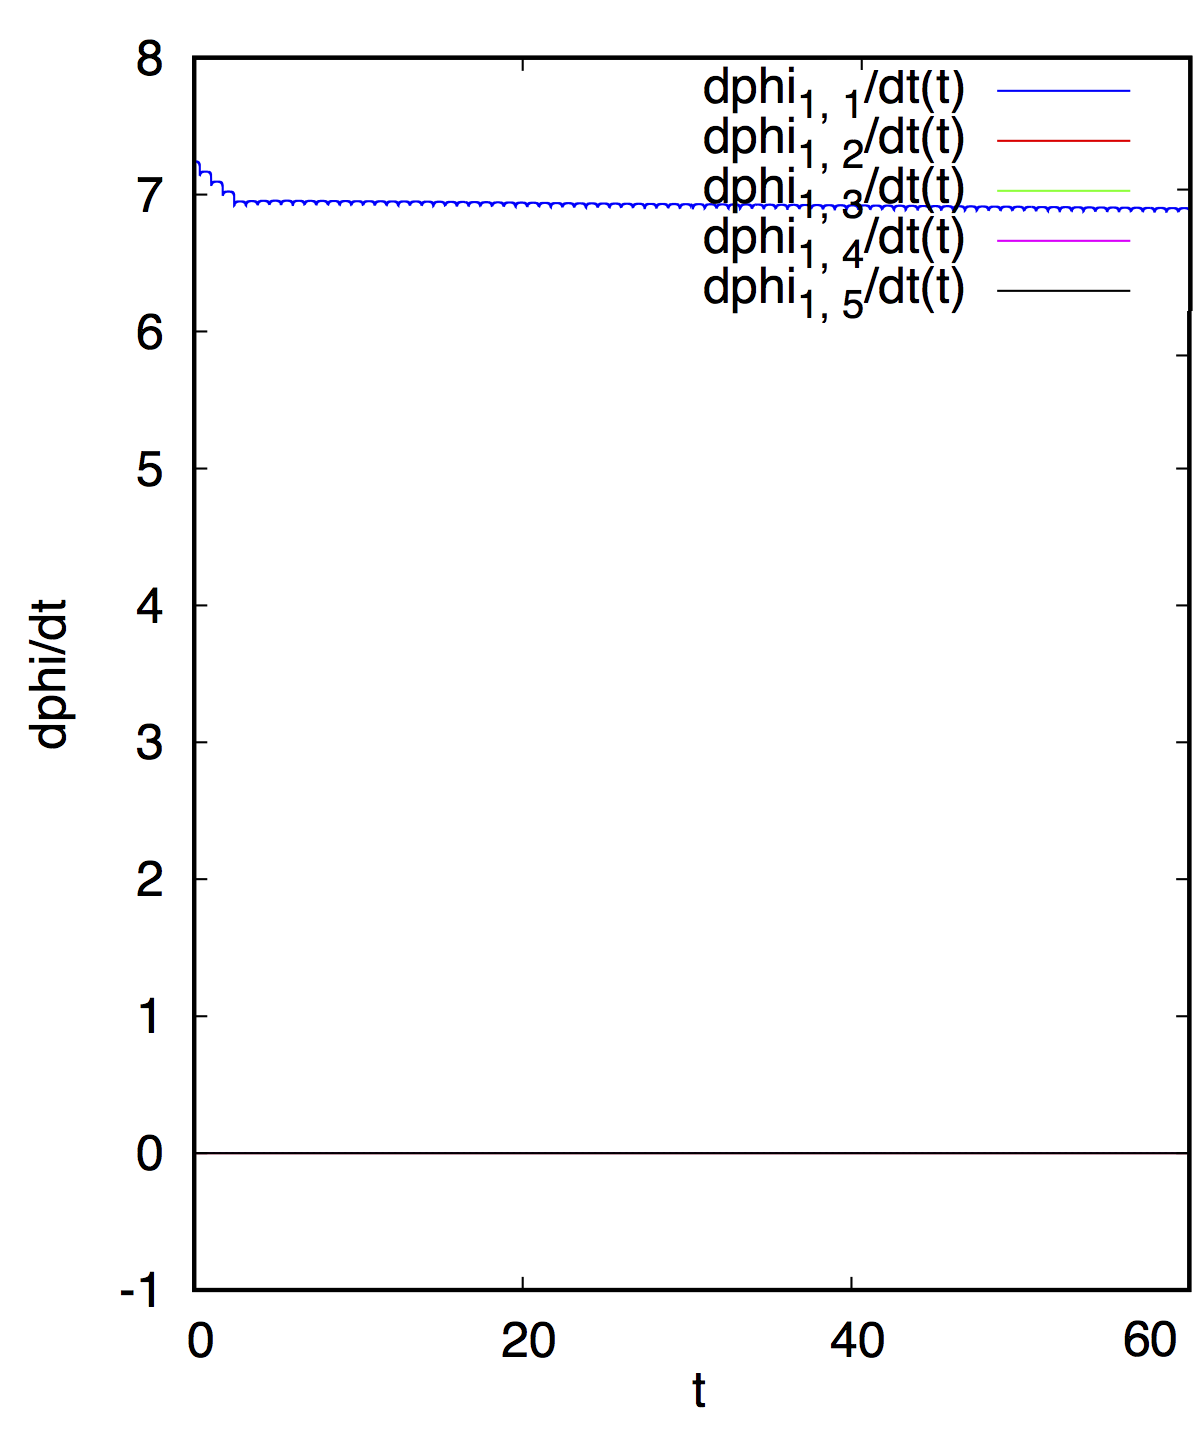
\includegraphics[width=0.8\linewidth]{content/pic/straight_60/nus1.png}
    %             \vspace{-15pt}
    %             \caption{$\dot{\mathbf{\phi}}$ на переднем колесе}
    %     \end{columns}
    % \end{figure}
    
    \centering
    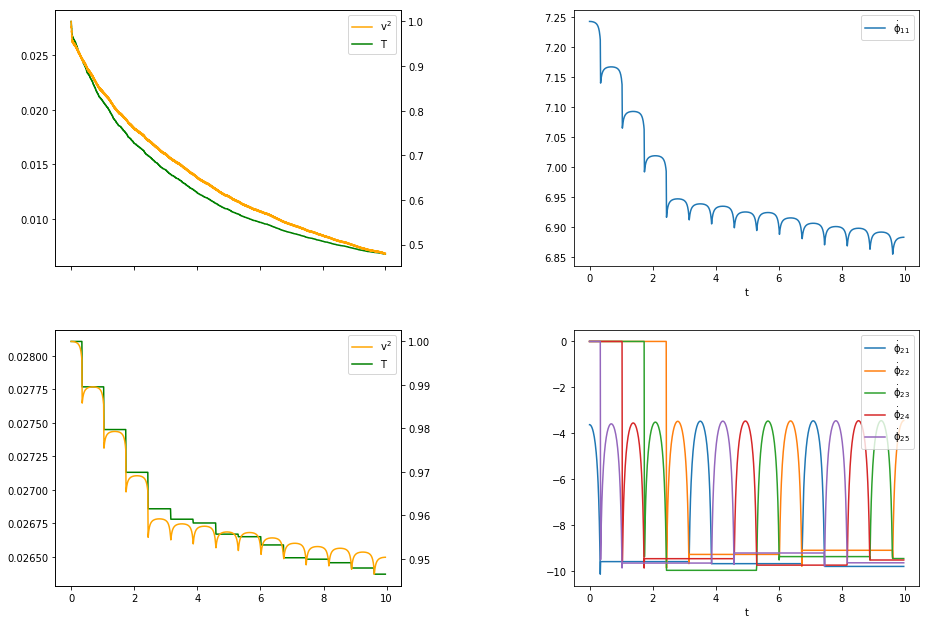
\includegraphics[width=\linewidth]{content/pic/new/impact_2.png}
    
\end{frame}

\begin{frame}{Движение 3 ($\nu_1(0) = 1, \nu_2(0) = 0, \nu_3(0) = 1$).}
%     \begin{figure}[H]
%         \centering
%         \begin{columns}
%             \column{0.33\textwidth}
%                 \centering
%                 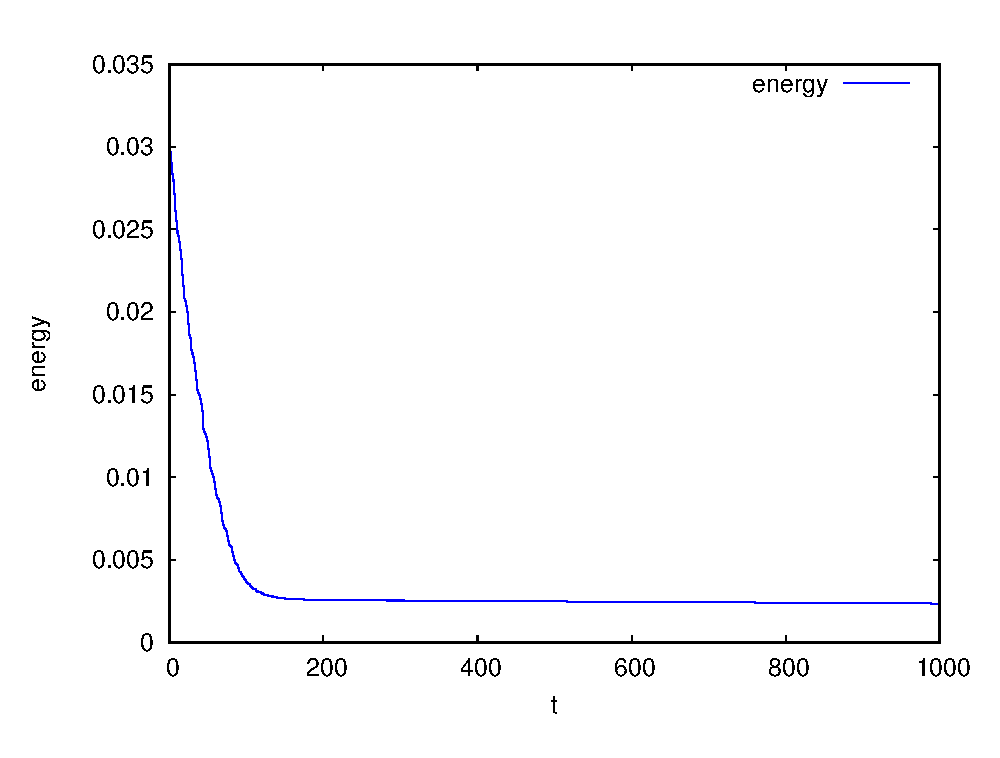
\includegraphics[width=\linewidth]{content/pic/wrench_1000/kin_en.eps}
%                 \vspace{-15pt}
%                 \caption{Кинетическая энергия}
%             \column{0.33\textwidth}
%                 \centering
%                 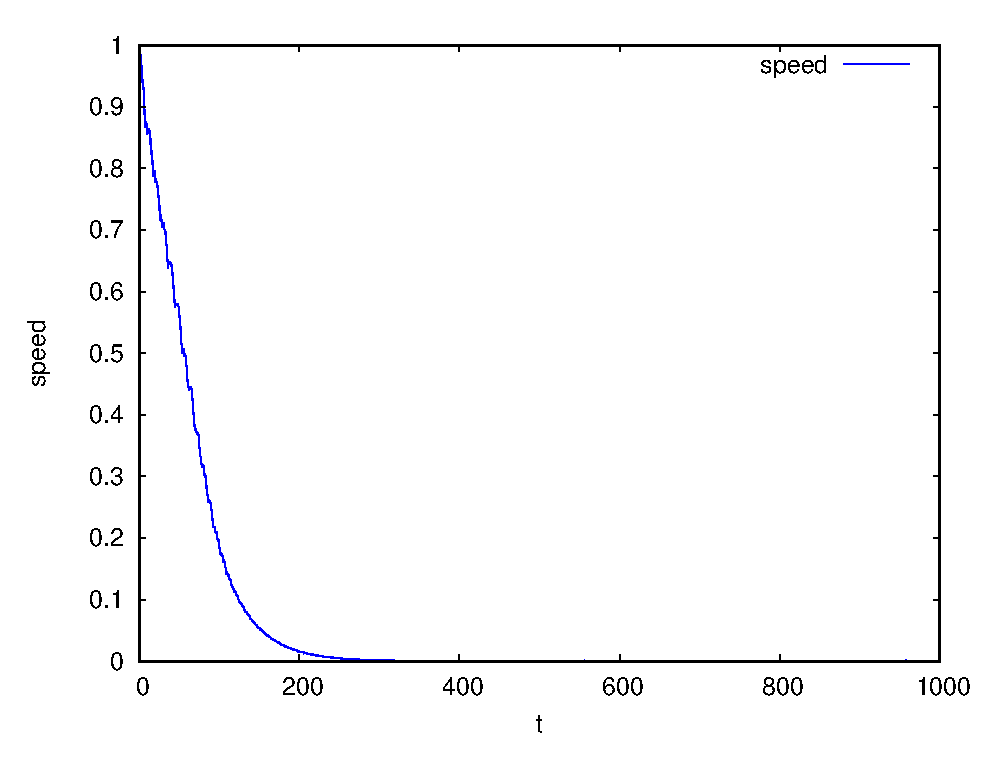
\includegraphics[width=\linewidth]{content/pic/wrench_1000/v.eps}
%                 \vspace{-15pt}
%                 \caption{Скорость центра масс}
%             \column{0.33\textwidth}
%                 \centering
%                 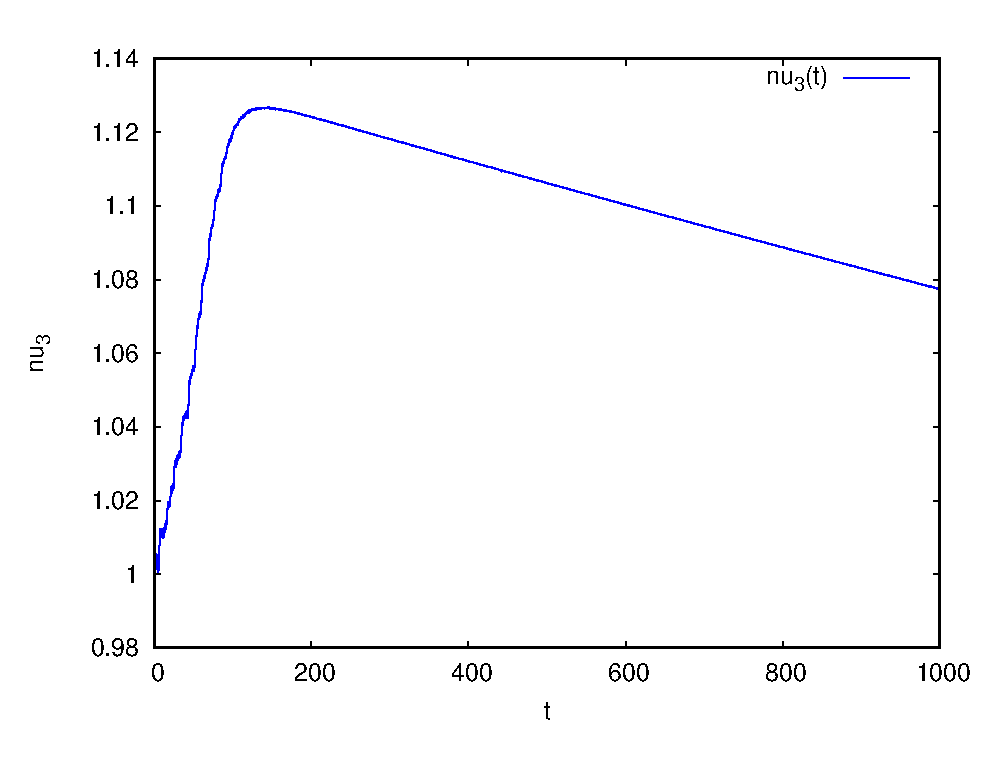
\includegraphics[width=\linewidth]{content/pic/wrench_1000/nu3.eps}
%                 \vspace{-15pt}
%                 \caption{Угловая скорость экипажа}
%         \end{columns}
%     \end{figure}
%     \vspace{-25pt}
%     \begin{figure}[H]
%         \centering
%         \begin{columns}
%             \column{0.33\textwidth}
%                 \centering
%                 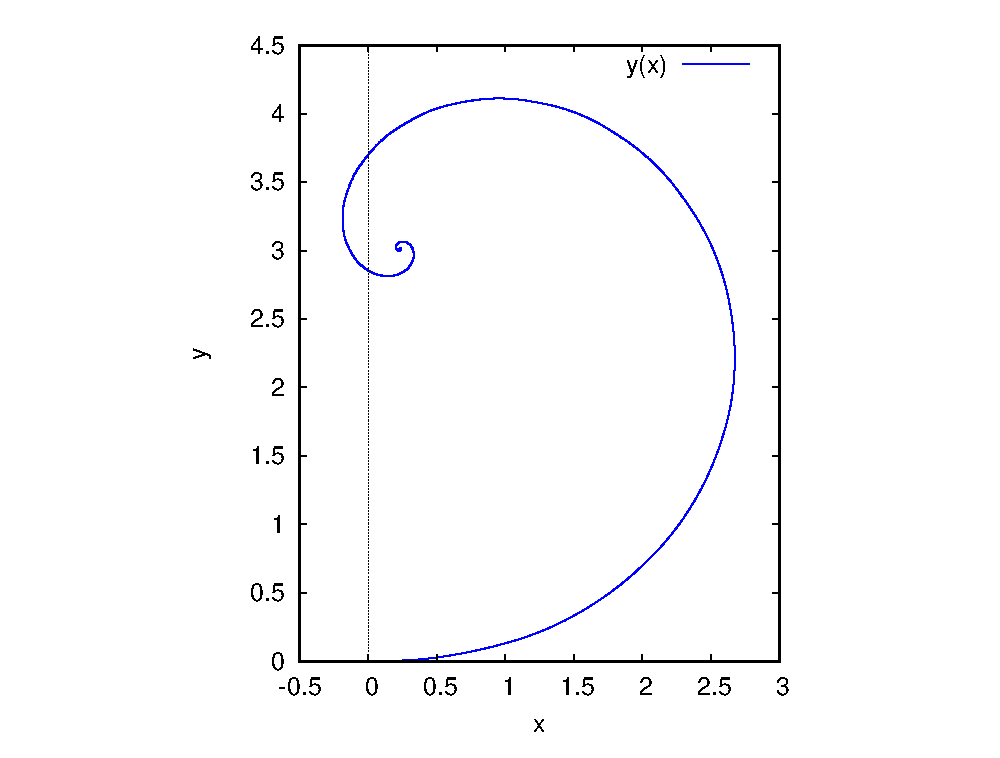
\includegraphics[width=\linewidth]{content/pic/wrench_1000/traj.eps}
%                 \vspace{-15pt}
%                 \caption{Траектория}
%             \column{0.33\textwidth}
%                 \centering
%                 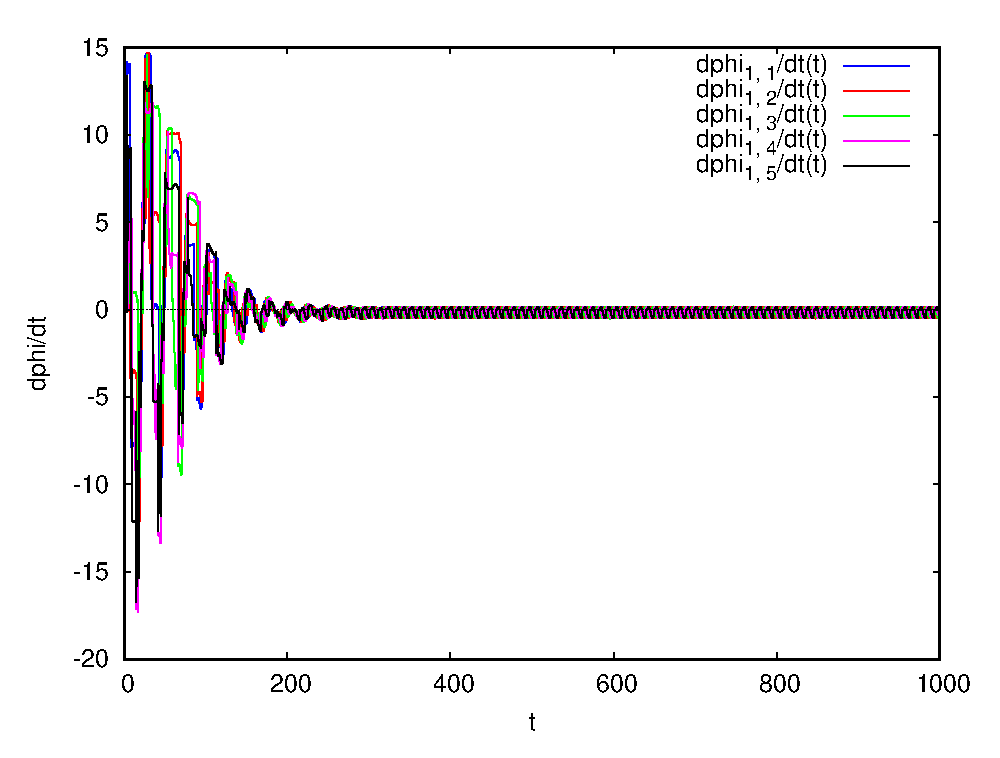
\includegraphics[width=\linewidth]{content/pic/wrench_1000/nus1.eps}
%                 \vspace{-15pt}
%                 \caption{$\dot{\mathbf{\phi}}$ на первом колесе}
%             % \column{0.33\textwidth}
%             %     \centering
%             %     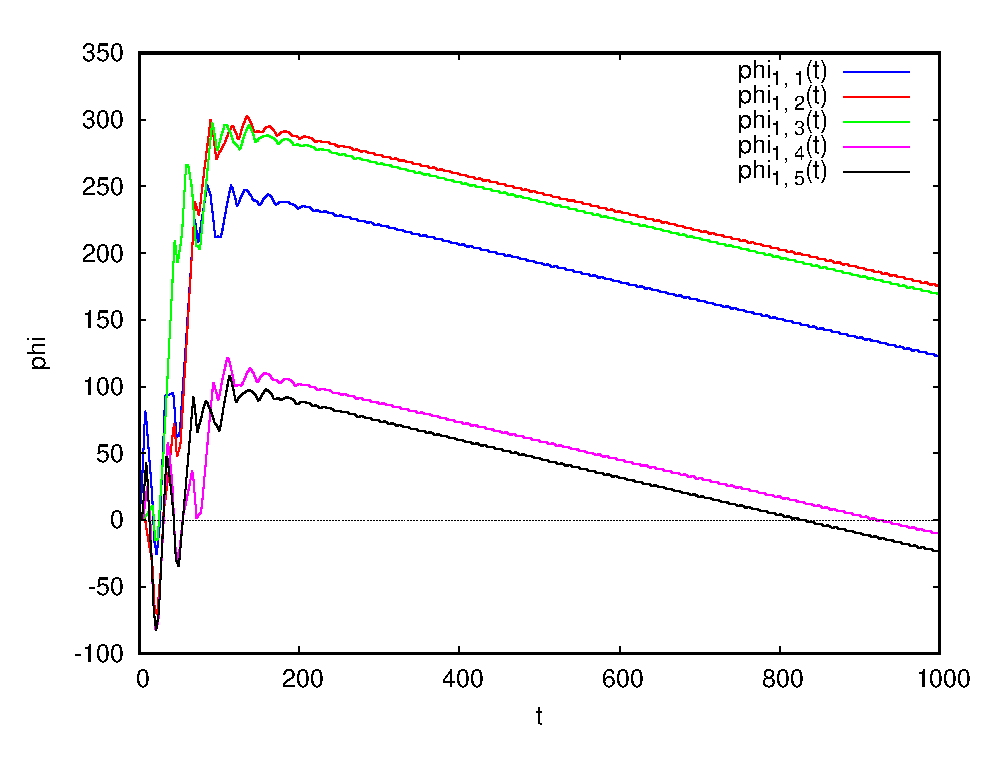
\includegraphics[width=\linewidth]{content/pic/wrench_1000/phi1.eps}
%             %     \vspace{-15pt}
%             %     \caption{углы$\mathbf{\phi}$ на первом колесе}
%         \end{columns}
%     \end{figure}
    \centering
    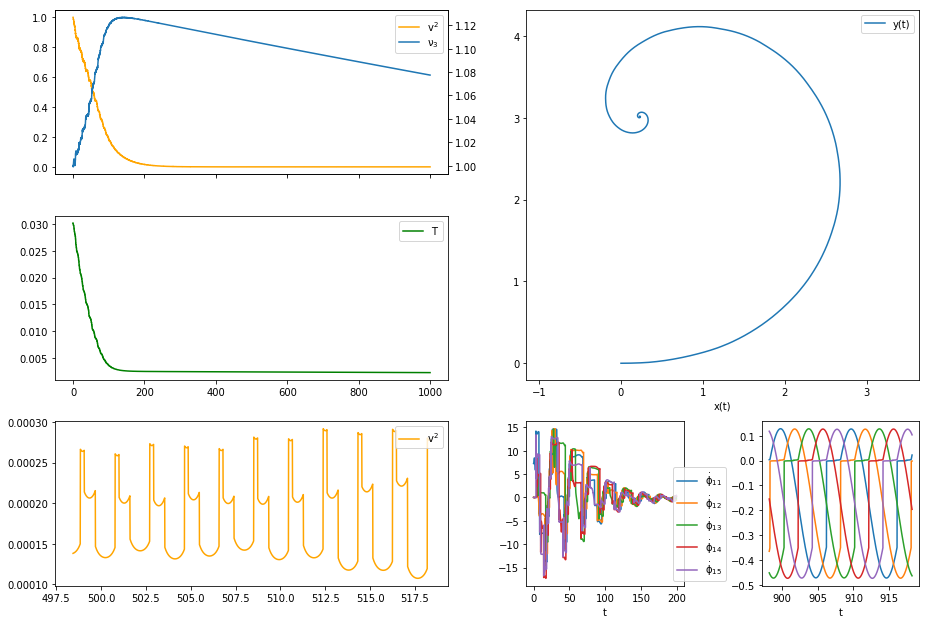
\includegraphics[width=\linewidth]{content/pic/new/impact_3.png}

\end{frame}
